\documentclass[11pt,letterpaper]{article}
\usepackage[utf8]{inputenc}
\usepackage[T1]{fontenc}
\usepackage[spanish]{babel}
\usepackage{amsmath,amssymb}
\usepackage{graphicx}
\usepackage{booktabs}
\usepackage{float}
\usepackage[margin=2.3cm]{geometry}
\usepackage{hyperref}
\usepackage{caption}
\captionsetup{font=small}
\graphicspath{{figures/}}
\setlength{\parskip}{0.5em}
\setlength{\parindent}{0pt}

% Pregunta literal del enunciado y respuesta directa
\newcommand{\preg}[1]{\par\medskip\noindent\textit{Enunciado: #1}\par}
\newcommand{\resp}[1]{\par\smallskip\noindent\fbox{\parbox{\dimexpr\linewidth-2\fboxsep-2\fboxrule\relax}{\textbf{Respuesta:} #1}}\par\medskip}

\title{Laboratorio 5: Modelo Espacial de Cobertura Hospitalaria\\
\large Respuestas de los Tasks 1 y 2 --- Estado de Texas}
\author{Humberto Alexander de la Cruz \and Daniel Oswaldo Juárez Herrera}
\date{CC2017 Modelación y Simulación}

\begin{document}
\maketitle

\section*{Selección del estado}
Se eligió \textbf{Texas} (código \texttt{TX}, FIPS 48). Es el estado con más hospitales con datos de camas (591, muy por encima del mínimo de 50) y tiene 254 condados que mezclan grandes áreas metropolitanas con extensas zonas rurales de baja densidad, lo que produce brechas de cobertura reales para analizar. Todo el código está en el notebook \texttt{lab5.ipynb}.

%=====================================================================
\section{Task 1}

%---------------------------------------------------------------------
\subsection{Task 1.1: Carga y preparación de datos}

\paragraph{a) Carga de los archivos.}
\preg{Cargue los cuatro archivos y, para cada uno, reporte número de registros, CRS y columnas disponibles. Incluya el código de carga en el apéndice.}
\resp{Los cuatro archivos se cargaron con GeoPandas (los tres GeoJSON) y Pandas (el CSV). Tienen 7,154 hospitales, 3,221 condados, 51 estados y 3,246 registros de población. Los tres GeoJSON están en EPSG:4326 y el CSV no tiene CRS. El código está en el Apéndice~\ref{app:carga} y las columnas en la tabla siguiente.}

\begin{table}[H]
\centering\small
\caption{Resumen de los cuatro archivos.}
\begin{tabular}{llrll}
\toprule
Archivo & Tipo & Registros & CRS & Columnas \\
\midrule
\texttt{hospitales\_eeuu.geojson} & GeoDataFrame & 7,154 & EPSG:4326 & \texttt{nombre, tipo, ciudad, estado, condado,} \\
 & & & & \texttt{fips\_condado, camas\_total, camas\_icu,} \\
 & & & & \texttt{camas\_licenciadas, ocupacion\_total,} \\
 & & & & \texttt{ocupacion\_icu, geometry} \\
\texttt{condados\_eeuu.geojson} & GeoDataFrame & 3,221 & EPSG:4326 & \texttt{fips, nombre, cod\_estado, geometry} \\
\texttt{estados\_eeuu.geojson} & GeoDataFrame & 51 & EPSG:4326 & \texttt{nombre, codigo, pais, geometry} \\
\texttt{poblacion\_condados.csv} & DataFrame & 3,246 & no aplica & \texttt{fips, condado, estado, lat, lon, poblacion} \\
\bottomrule
\end{tabular}
\end{table}

\paragraph{b) Limpiezas previas al filtro por estado.}
\preg{Elimine los registros con $\text{FIPS}\ge80000$ y convierta \texttt{fips} a \emph{string} de cinco dígitos. Reporte qué porcentaje de hospitales tiene \texttt{camas\_total} nulo, trabaje solo con los que tienen datos y documente cuántos quedan en el estado elegido.}
\resp{El \textbf{15.24\,\%} de los hospitales tiene \texttt{camas\_total} nulo. Se eliminaron 102 registros de población con $\text{FIPS}\ge80000$ y \texttt{fips} quedó como \emph{string} de cinco dígitos. En Texas quedan \textbf{591} hospitales con datos de camas (de 739).}
\begin{itemize}
  \item \textbf{Población:} se eliminaron los registros con $\text{FIPS}\ge 80000$ (3,246 $\to$ 3,144 registros; se descartaron 102). La columna \texttt{fips} se convirtió a \emph{string} de cinco dígitos con \texttt{zfill(5)}.
  \item \textbf{Hospitales:} el \textbf{15.24\,\%} de los registros (1,090 de 7,154) tiene \texttt{camas\_total} nulo. Se trabajó solo con los 6,064 hospitales con datos de camas. En Texas hay 739 hospitales en total y \textbf{591} quedan después de la limpieza.
\end{itemize}

\paragraph{c) Filtro por estado y unión.}
\preg{Filtre hospitales y condados para el estado elegido, una la población con la geometría por FIPS y verifique que el número de condados con geometría y con población coincida.}
\resp{Sí coinciden: hay \textbf{254 condados con geometría y 254 con población}, y los 254 se unieron sin valores nulos.}
Hospitales: \texttt{estado == "TX"}. Condados: \texttt{cod\_estado == "48"}. La unión con la población se hizo por \texttt{fips}. Hay \textbf{254 condados con geometría y 254 con población, y los 254 coinciden}. La población total de Texas es de \textbf{28,995,881} habitantes.

\paragraph{d) Reproyección y justificación del CRS.}
\preg{Reproyecte todas las capas a un CRS proyectado apropiado para el estado y justifique formalmente la elección con su código EPSG y la razón por la que minimiza la distorsión.}
\resp{Se usó \textbf{EPSG:3083} (NAD83 / Texas Centric Albers Equal Area) porque es el sistema diseñado para todo Texas, conserva el área y su distorsión lineal es de $\approx\pm0.22\,\%$ en cualquier punto del estado (detalle abajo).}
Todas las capas se reproyectaron a EPSG:3083.
\begin{itemize}
  \item Es el sistema del \emph{Texas Centric Mapping System}, diseñado para cubrir \textbf{todo el estado con una sola proyección}. UTM obligaría a partir Texas en las zonas 13, 14 y 15, y usar una sola zona (por ejemplo la 14N) daría un factor de escala de 1.006 (0.6\,\%) y un factor de área de 1.012 en el extremo oeste, casi tres veces la distorsión de Albers.
  \item Es una proyección \textbf{cónica de áreas iguales} (Albers) con paralelos estándar en $27.5^\circ$\,N y $35^\circ$\,N y meridiano central en $100^\circ$\,O. Los factores de escala calculados en las esquinas y el centro del estado dan una distorsión lineal de $\approx\pm0.22\,\%$ ($k$ entre 0.9978 y 1.0022), es decir $\approx 55$\,m en un buffer de 25\,km y $\approx 110$\,m en uno de 50\,km.
  \item \textbf{Conserva el área} (factor de área igual a 1.0000 en todos los puntos). Esto es conveniente porque la fórmula de población cubierta usa cocientes de áreas $\text{Área}(\text{Condado}_i\cap\text{Buffer})/\text{Área}(\text{Condado}_i)$, que resultan exactos bajo el supuesto de población uniforme.
  \item La alternativa conforme (EPSG:3081, Lambert) tiene la misma distorsión lineal, pero deforma las áreas hasta $\approx0.4\,\%$. Por eso se prefirió Albers.
\end{itemize}

\paragraph{e) Mapa base.}
\preg{Genere un mapa de tres capas: condados en gris claro, hospitales como puntos de color según su tipo y el límite estatal como contorno sin relleno, con escala gráfica y título.}
\resp{El mapa (Figura siguiente) muestra los 254 condados en gris, los 591 hospitales coloreados por \texttt{tipo} (309 son \emph{General Acute Care}) y el límite de Texas sin relleno, con escala gráfica y título.}
\begin{figure}[H]
\centering
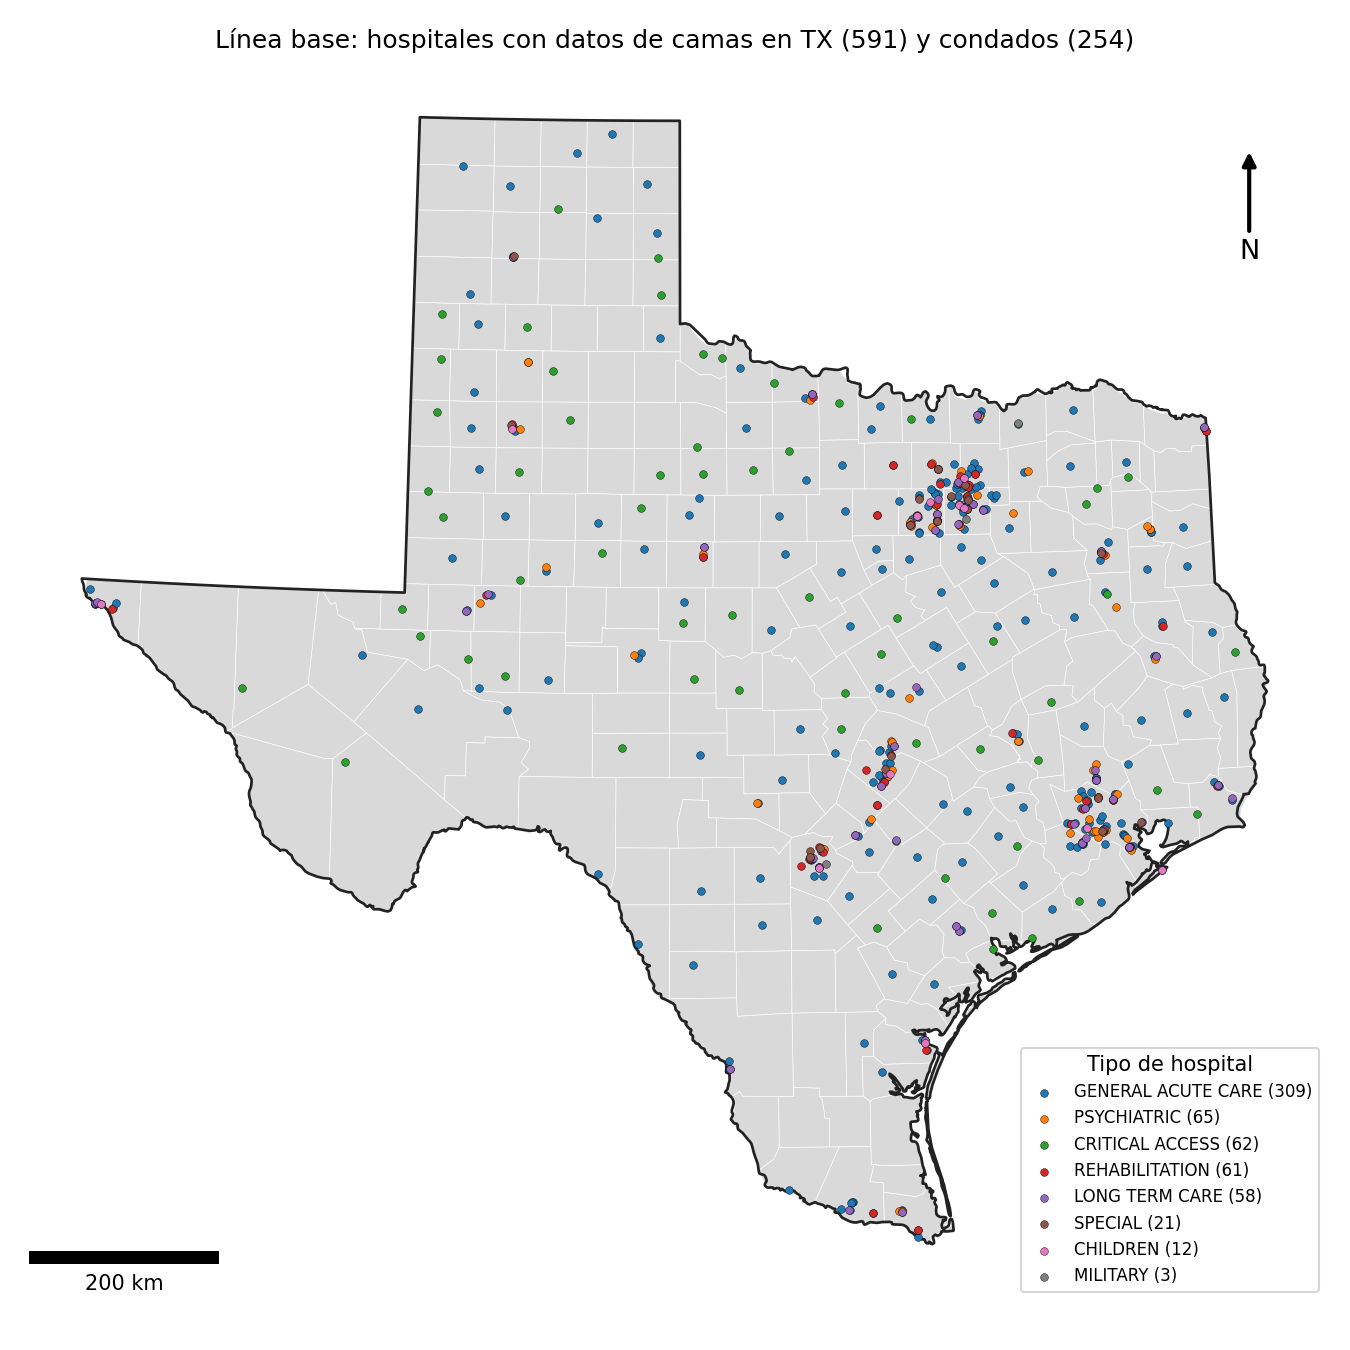
\includegraphics[width=0.85\textwidth]{mapa_base.png}
\caption{Línea base: condados (gris claro), hospitales por tipo (puntos de color) y límite estatal (contorno sin relleno).}
\end{figure}

%---------------------------------------------------------------------
\subsection{Task 1.2: Análisis estadístico y distribución por condado}

\preg{Calcule y reporte en una tabla, por condado: número de hospitales, camas totales, camas UCI, población total, camas totales por cada 10,000 habitantes y camas UCI por cada 10,000 habitantes. Asigne cero a los condados sin hospitales.}
\resp{La tabla de los 254 condados se calculó con esas seis columnas (con ceros para los 77 condados sin hospitales) y está completa en el notebook; aquí se muestran los cinco más poblados.}
La tabla completa de los 254 condados (hospitales, camas totales, camas UCI, población, camas por 10,000 habitantes y camas UCI por 10,000 habitantes, con ceros para condados sin hospitales) está en el notebook. Texas tiene 72,752 camas en total y \textbf{77 condados sin ningún hospital} con datos de camas. A modo de ejemplo, los cinco condados más poblados:

\begin{table}[H]
\centering\small
\caption{Estadísticas por condado (cinco más poblados).}
\begin{tabular}{lrrrrrr}
\toprule
Condado & Población & Hospitales & Camas & Camas UCI & Camas/10k & UCI/10k \\
\midrule
Harris  & 4,713,325 & 61 & 13,411 & 1,242 & 28.45 & 2.64 \\
Dallas  & 2,635,516 & 42 & 7,459  & 613   & 28.30 & 2.33 \\
Tarrant & 2,102,515 & 44 & 5,612  & 461   & 26.69 & 2.19 \\
Bexar   & 2,003,554 & 27 & 6,406  & 561   & 31.97 & 2.80 \\
Travis  & 1,273,954 & 22 & 3,112  & 309   & 24.43 & 2.43 \\
\bottomrule
\end{tabular}
\end{table}

\paragraph{a) Cinco condados con menos camas por habitante (población $>10{,}000$).}
\preg{Identifique los cinco condados con menor cantidad de camas por habitante entre los condados con población mayor a 10,000 habitantes.}
\resp{Randall, Orange, San Patricio, Hardin y Van Zandt. Los cinco tienen 0 camas (no tienen hospitales con datos de camas); se desempató por mayor población.}
Hay 166 condados con más de 10,000 habitantes, y 31 de ellos no tienen hospitales. Como todos estos empatan en 0 camas, se desempató por mayor población.

\begin{table}[H]
\centering\small
\begin{tabular}{lrrrr}
\toprule
Condado & Población & Hospitales & Camas & Camas/10k \\
\midrule
Randall      & 137,713 & 0 & 0 & 0.00 \\
Orange       & 83,396  & 0 & 0 & 0.00 \\
San Patricio & 66,730  & 0 & 0 & 0.00 \\
Hardin       & 57,602  & 0 & 0 & 0.00 \\
Van Zandt    & 56,590  & 0 & 0 & 0.00 \\
\bottomrule
\end{tabular}
\end{table}

Los cinco son condados de tamaño medio sin ningún hospital con datos de camas. ``Cero camas en el condado'' no significa ``cero acceso'': su población probablemente usa hospitales de condados vecinos, y esa distancia se mide en el Task 2.1.

\paragraph{b) Cinco condados con mayor concentración de camas.}
\preg{Identifique los cinco condados con mayor concentración de camas por habitante. Argumente si esa concentración representa una ventaja de acceso para la población del condado o puede reflejar otro fenómeno, como hospitales regionales que atienden a condados vecinos.}
\resp{Los cinco son Stonewall (148.15 camas/10k), Hardeman (114.42), Throckmorton (93.27), Fannin (89.26) y Wheeler (81.09). \textbf{No representa una ventaja de acceso}: refleja principalmente poblaciones diminutas (un hospital pequeño basta para una razón alta) y, en el caso de Fannin, un hospital regional de veteranos de 292 camas que atiende a una región amplia. Son hospitales que sirven también a condados vecinos.}
\begin{table}[H]
\centering\small
\begin{tabular}{lrrrrrr}
\toprule
Condado & Población & Hospitales & Camas & Camas/10k & Mayor hospital & Pob. vecinos $\le$50\,km \\
\midrule
Stonewall    & 1,350  & 1 & 20  & 148.15 & 20  & 6,692 \\
Hardeman     & 3,933  & 2 & 45  & 114.42 & 24  & 1,155 \\
Throckmorton & 1,501  & 1 & 14  & 93.27  & 14  & 27,177 \\
Fannin       & 35,514 & 2 & 317 & 89.26  & 292 & 5,331 \\
Wheeler      & 5,056  & 2 & 41  & 81.09  & 25  & 28,625 \\
\bottomrule
\end{tabular}
\end{table}

En su mayoría esta concentración es un \textbf{artefacto del denominador} y no una ventaja real de acceso:
\begin{itemize}
  \item Cuatro de los cinco (Stonewall, Hardeman, Throckmorton y Wheeler) son condados rurales con entre 1,350 y 5,056 habitantes. Uno o dos hospitales pequeños (14 a 45 camas en total, típicos de hospitales de acceso crítico) bastan para dar 81 a 148 camas por 10,000 habitantes simplemente porque la población es diminuta. Eso no implica más servicios.
  \item Esos hospitales atienden también a los habitantes de condados vecinos, que a su vez no tienen hospital.
  \item \textbf{Fannin} es distinto: su mayor hospital tiene 292 camas y corresponde al \emph{Sam Rayburn Memorial Veterans Center} (tipo \texttt{MILITARY}), un hospital de veteranos que atiende una región amplia y no solo al condado. Es un caso claro de hospital regional que infla el indicador.
\end{itemize}
Por tanto, las camas por habitante a nivel condado mezclan capacidad real con tamaño de población y con flujos entre condados, y conviene complementarlas con medidas de distancia.

\paragraph{c) Distribuciones.}
\preg{Grafique el histograma de camas por hospital y el de camas por habitante por condado. Interprete la forma de cada distribución: ¿son simétricas, asimétricas, tienen valores extremos? ¿Qué implica eso para el análisis de cobertura?}
\resp{\textbf{Ninguna es simétrica; las dos son asimétricas a la derecha y tienen valores extremos.} Camas por hospital: asimetría 3.67, media 123 contra mediana 54, máximo 1,560. Camas por 10,000 habitantes por condado: asimetría 1.90, pico en cero (77 de 254 condados) y valores extremos de hasta 148. Implicaciones: la media no es representativa, las razones por habitante se degradan en condados con cero camas o población muy pequeña, y un buffer trata igual a un hospital de 3 camas que a uno de 1,560, de modo que la cobertura por distancia sobrestima la capacidad efectiva.}
\begin{figure}[H]
\centering
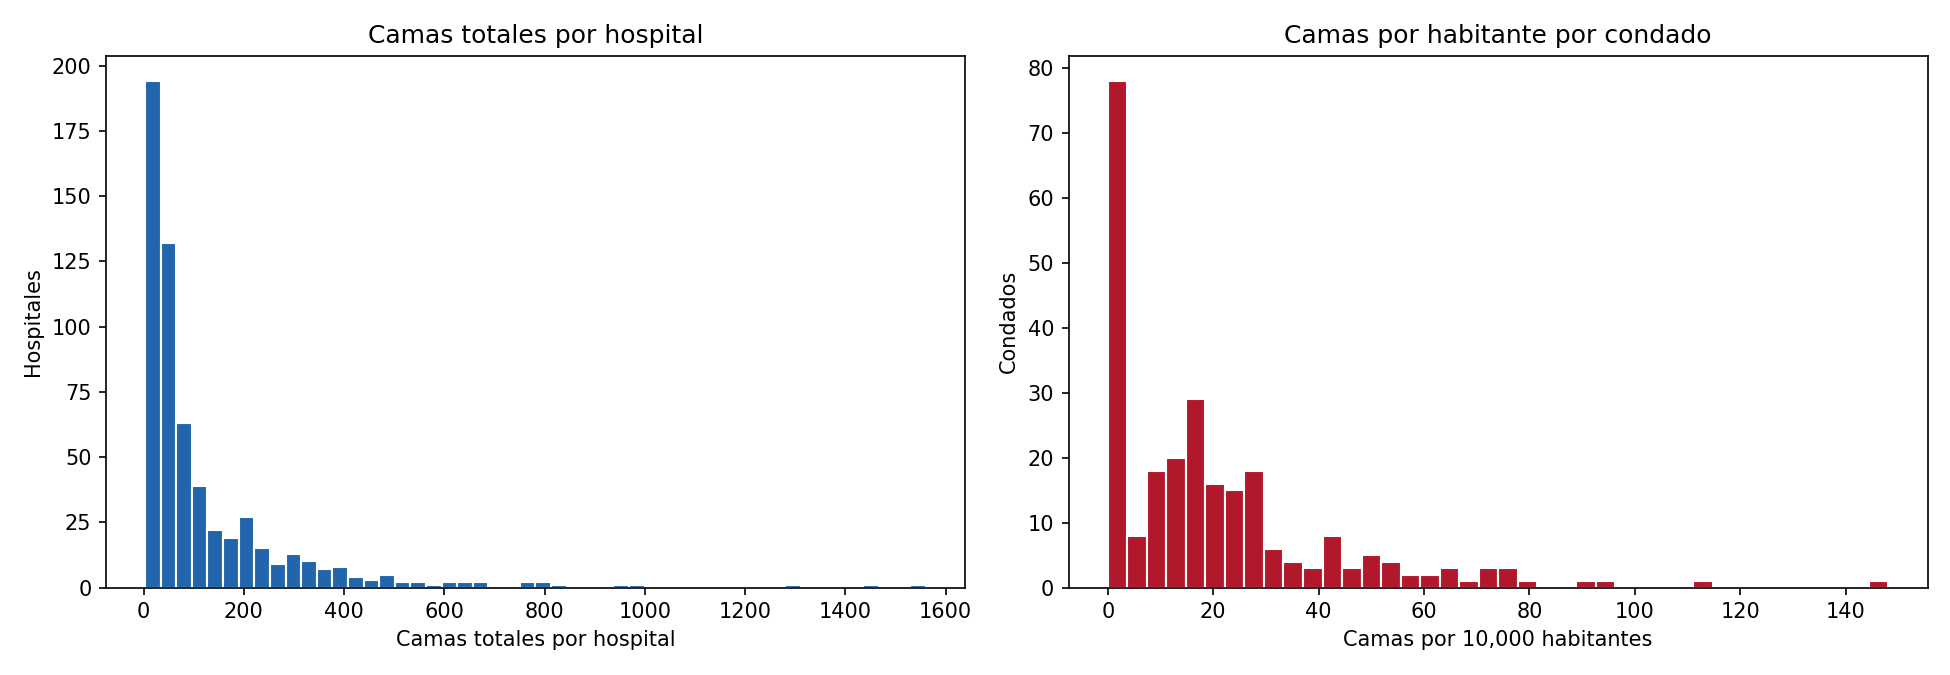
\includegraphics[width=0.95\textwidth]{histogramas.png}
\caption{Izquierda: camas totales por hospital. Derecha: camas por 10,000 habitantes por condado.}
\end{figure}

\begin{itemize}
  \item \textbf{Camas por hospital:} muy asimétrica a la derecha (asimetría 3.67). La media (123.1) es más del doble que la mediana (54) y el máximo es 1,560. 392 de los 591 hospitales tienen menos de 100 camas. Pocos hospitales muy grandes concentran gran parte de la capacidad.
  \item \textbf{Camas por 10,000 habitantes por condado:} también asimétrica a la derecha (asimetría 1.90; media 19.7, mediana 15.0, máximo 148.1) y con un \textbf{pico en cero}: 77 de 254 condados (30\,\%) no tienen camas. De los 177 condados con camas, 121 están entre 5 y 30 y hay valores extremos que corresponden a condados diminutos.
  \item \textbf{Implicaciones para la cobertura:} (i) la media no es representativa y conviene usar medianas o percentiles; (ii) los condados con cero camas hacen que las razones por habitante estén indefinidas o saturadas; (iii) un buffer cuenta igual a un hospital de 3 camas que a uno de 1,560, de modo que la cobertura por distancia \textbf{sobrestima la cobertura efectiva de capacidad}; (iv) los valores extremos pueden dominar cualquier promedio sin transformar.
\end{itemize}

%---------------------------------------------------------------------
\subsection{Task 1.3: Análisis de buffer de cobertura poblacional}

\paragraph{a) Buffers.}
\preg{Genere buffers circulares de 10, 25 y 50\,km alrededor de cada hospital en las capas reproyectadas y una los buffers del mismo radio con \texttt{unary\_union}.}
\resp{Se generaron los tres conjuntos de buffers en EPSG:3083 y se unieron con \texttt{unary\_union}. Las áreas unificadas son 83,209, 363,435 y 667,115\,km$^2$ para 10, 25 y 50\,km.}
Para cada radio $r\in\{10,25,50\}$\,km se generó un buffer circular alrededor de cada hospital en la capa proyectada (metros) y se unieron con \texttt{unary\_union}:
\[
C_r=\bigcup_{h} B(h,r).
\]
El área de cobertura unificada es 83,209\,km$^2$ para 10\,km, 363,435\,km$^2$ para 25\,km y 667,115\,km$^2$ para 50\,km (el área de Texas es 685,340\,km$^2$; la unión incluye zonas fuera del estado).

\paragraph{b) Población cubierta.}
\preg{Para cada radio, calcule la fracción de la población total del estado que queda dentro del área de cobertura unificada, asumiendo población uniforme en cada condado, y reporte una tabla con radio, población cubierta estimada, población total y porcentaje de cobertura.}
\resp{La cobertura es \textbf{47.08\,\% a 10\,km, 87.30\,\% a 25\,km y 98.98\,\% a 50\,km} de los 28,995,881 habitantes (tabla siguiente).}
Con población uniforme dentro de cada condado,
\[
\text{Población Cubierta}_i=\text{Población}_i\times\frac{\text{Área}(\text{Condado}_i\cap\text{Buffer})}{\text{Área}(\text{Condado}_i)}.
\]

\begin{table}[H]
\centering\small
\begin{tabular}{rrrr}
\toprule
Radio (km) & Población cubierta estimada & Población total & Cobertura (\%) \\
\midrule
10 & 13,652,045 & 28,995,881 & 47.08 \\
25 & 25,312,722 & 28,995,881 & 87.30 \\
50 & 28,698,735 & 28,995,881 & 98.98 \\
\bottomrule
\end{tabular}
\end{table}

La cobertura por población crece mucho más rápido que la cobertura por área (a 25\,km se cubre el 87\,\% de la gente pero solo $\approx51\,\%$ del territorio del estado), porque la población se concentra en las áreas metropolitanas, donde hay muchos hospitales.

\paragraph{c) Mapa a 25 km.}
\preg{Genere un mapa de cobertura para 25\,km con los condados coloreados como completamente cubiertos, parcialmente cubiertos o no cubiertos, los hospitales superpuestos y una escala de color divergente que resalte las zonas sin cobertura.}
\resp{A 25\,km hay \textbf{8 condados completamente cubiertos, 233 parcialmente cubiertos y 13 no cubiertos} (Figura siguiente; los no cubiertos en rojo).}
De los 254 condados, 8 están completamente cubiertos, 233 parcialmente cubiertos y 13 no cubiertos (se consideró ``completamente cubierto'' una fracción de área $\ge0.999$).
\begin{figure}[H]
\centering
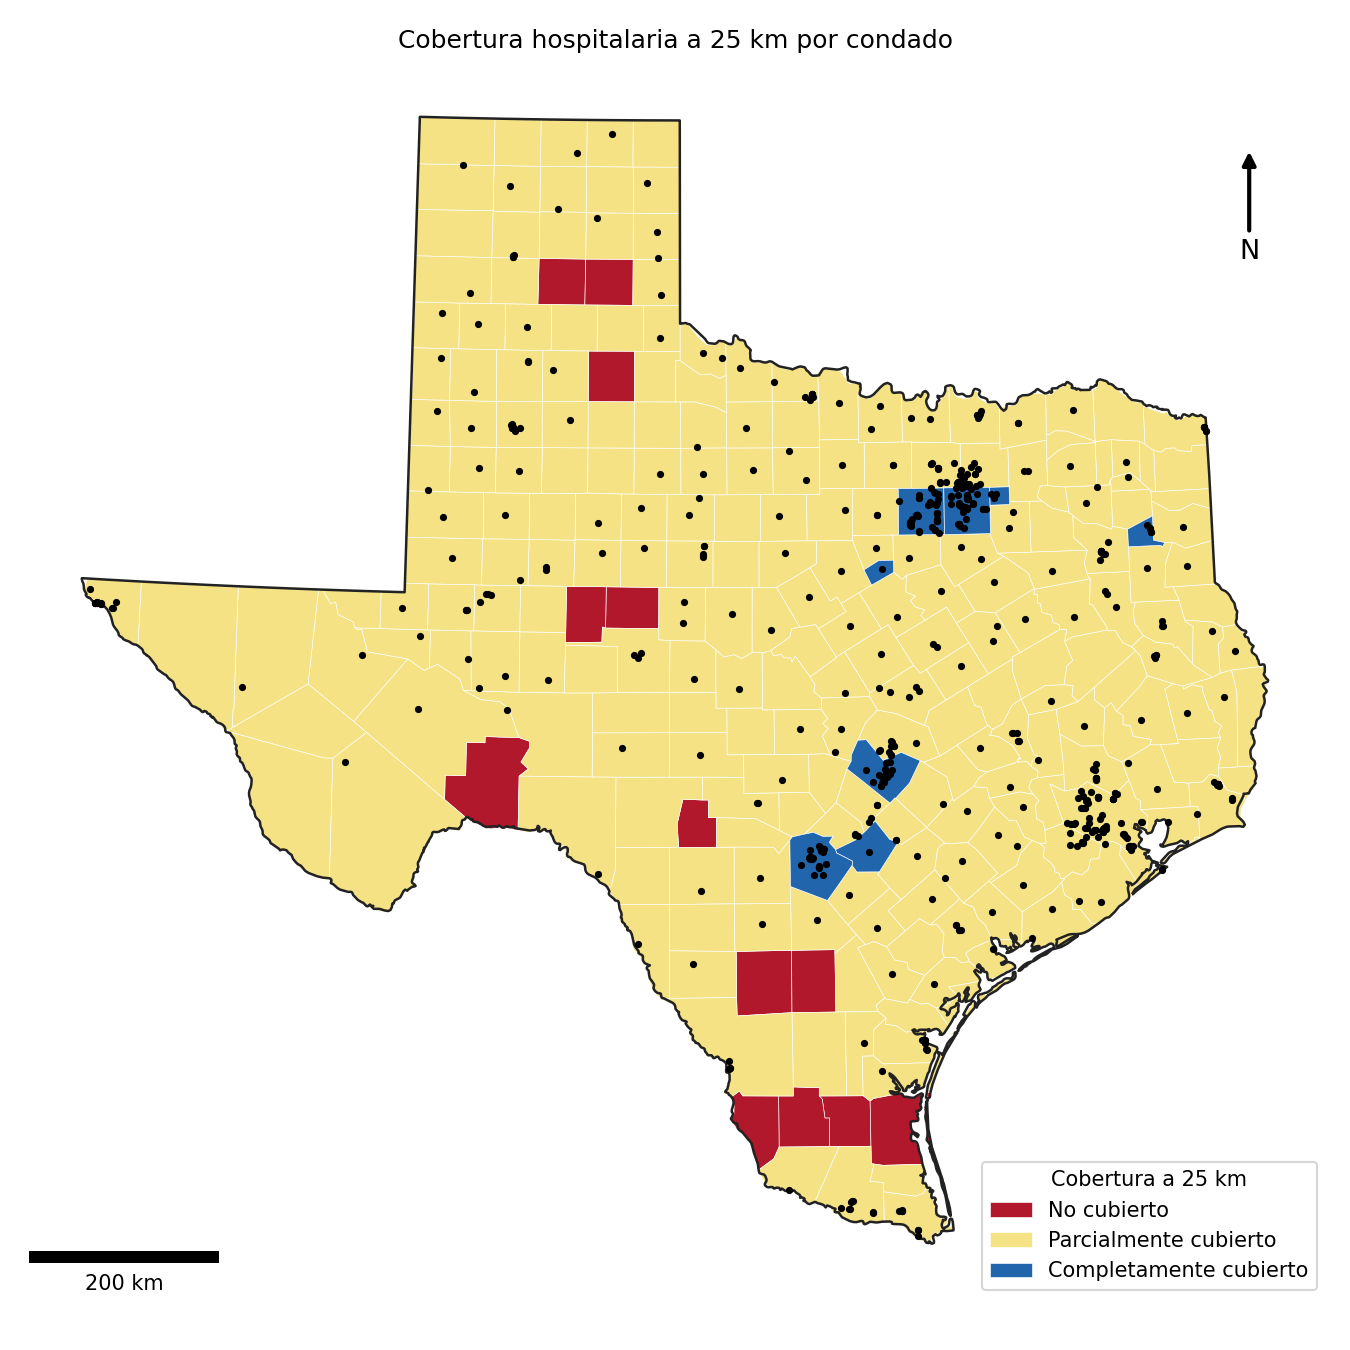
\includegraphics[width=0.85\textwidth]{cobertura_25km.png}
\caption{Cobertura a 25\,km por condado (escala divergente: rojo = no cubierto).}
\end{figure}

%=====================================================================
\section{Task 2}

%---------------------------------------------------------------------
\subsection{Task 2.1: Sensibilidad del análisis de distancia}

\paragraph{a) Diez condados más lejos del hospital más cercano.}
\preg{Para cada condado calcule la distancia en kilómetros al hospital más cercano usando el centroide como punto de referencia. Reporte los diez condados con mayor distancia.}
\resp{Los diez más alejados son Terrell (78.6\,km), Jim Hogg (75.5), Brewster (75.4), Edwards (71.9), Hudspeth (69.8), Presidio (69.4), Real (68.4), Zapata (66.3), Kenedy (65.2) y Oldham (65.0). Todos están a más de 65\,km de un hospital.}
Distancia del centroide del condado, en la capa proyectada:

\begin{table}[H]
\centering\small
\begin{tabular}{llrr}
\toprule
\# & Condado & Población & Distancia (km) \\
\midrule
1 & Terrell  & 776    & 78.6 \\
2 & Jim Hogg & 5,200  & 75.5 \\
3 & Brewster & 9,203  & 75.4 \\
4 & Edwards  & 1,932  & 71.9 \\
5 & Hudspeth & 4,886  & 69.8 \\
6 & Presidio & 6,704  & 69.4 \\
7 & Real     & 3,452  & 68.4 \\
8 & Zapata   & 14,179 & 66.3 \\
9 & Kenedy   & 404    & 65.2 \\
10 & Oldham  & 2,112  & 65.0 \\
\bottomrule
\end{tabular}
\end{table}

Son condados muy poco poblados (de 404 a 14,179 habitantes) concentrados en el sur, hacia la frontera con México (Jim Hogg, Zapata, Kenedy), y en el oeste y suroeste (Terrell, Edwards, Real, Brewster, Presidio, Hudspeth), más Oldham en el \emph{Panhandle}. Como la distancia se mide desde el centroide, es una aproximación.

\paragraph{b) Curva de cobertura acumulada (5 a 100 km, pasos de 5 km).}
\preg{Grafique el porcentaje de población cubierta para radios de 5 a 100\,km en pasos de 5\,km, identifique el punto de inflexión donde la cobertura deja de crecer rápidamente y argumente qué significa ese punto para la política de acceso hospitalario en el estado.}
\resp{El punto de inflexión está en \textbf{30\,km, con 93.2\,\% de la población cubierta}. Significa que la red actual ya cubre a casi toda la población en distancias cortas y que el $\approx7\,\%$ restante (unos 2 millones de personas) vive en zonas muy poco pobladas, donde más hospitales fijos rinden muy poco: la política debe pasar de ``más cobertura'' a intervenciones distintas (transporte de emergencia, telemedicina, clínicas móviles, hospitales de acceso crítico mejor equipados).}

\begin{table}[H]
\centering\footnotesize
\begin{tabular}{l*{10}{r}}
\toprule
Radio (km) & 5 & 10 & 15 & 20 & 25 & 30 & 35 & 40 & 45 & 50 \\
Cobertura (\%) & 22.77 & 47.08 & 63.51 & 77.28 & 87.30 & 93.20 & 96.13 & 97.61 & 98.44 & 98.98 \\
Ganancia (pp) & -- & 24.31 & 16.43 & 13.77 & 10.02 & 5.90 & 2.93 & 1.48 & 0.83 & 0.53 \\
\midrule
Radio (km) & 55 & 60 & 65 & 70 & 75 & 80 & 85 & 90 & 95 & 100 \\
Cobertura (\%) & 99.37 & 99.63 & 99.74 & 99.83 & 99.89 & 99.92 & 99.94 & 99.96 & 99.97 & 99.98 \\
Ganancia (pp) & 0.40 & 0.25 & 0.12 & 0.09 & 0.05 & 0.03 & 0.02 & 0.02 & 0.01 & 0.01 \\
\bottomrule
\end{tabular}
\end{table}

\begin{figure}[H]
\centering
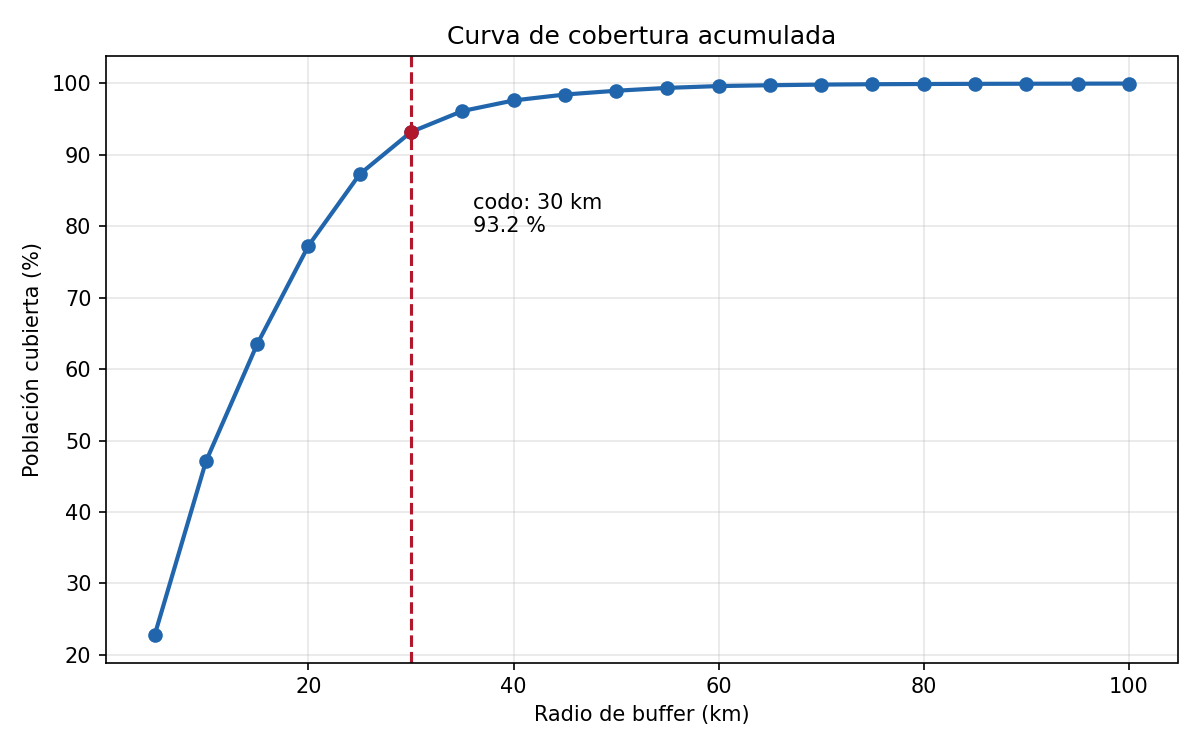
\includegraphics[width=0.7\textwidth]{curva_cobertura.png}
\caption{Curva de cobertura acumulada con el punto de inflexión (método del codo).}
\end{figure}

El punto de inflexión, calculado con el método del codo (máxima separación entre la curva normalizada y la diagonal), está en \textbf{30\,km, con 93.2\,\% de la población cubierta}. Hasta ese radio cada 5\,km adicionales suman entre 24 y 6 puntos porcentuales; después suman menos de 3 puntos, y pasados 50\,km, menos de 0.5.

\textbf{Significado para la política de acceso hospitalario en Texas:}
\begin{itemize}
  \item La red actual ya llega a $\approx93\,\%$ de la población dentro de 30\,km (unos 30 a 40 minutos por carretera): el problema no es la cobertura general.
  \item El $\approx7\,\%$ restante ($\approx2$ millones de personas) vive en zonas de muy baja densidad. Alcanzarlo con hospitales fijos exigiría construir en lugares casi vacíos, con un costo por persona muy alto.
  \item Por tanto, ampliar la cobertura de las zonas remotas requiere \textbf{otro tipo de intervención} (transporte de emergencia y aéreo, telemedicina, clínicas móviles, hospitales de acceso crítico bien equipados) y no más hospitales convencionales.
  \item Es una lectura de cobertura por distancia en línea recta: no dice nada sobre la capacidad ni sobre el tiempo real de viaje.
\end{itemize}

\paragraph{c) Tipo del hospital más cercano a los cinco condados más alejados.}
\preg{Para los cinco condados con mayor distancia, calcule qué tipo de hospital es el más cercano. ¿Los condados más alejados tienden a estar cerca de hospitales de menor capacidad? Apoye su respuesta con los datos de camas del hospital más cercano.}
\resp{\textbf{Sí.} Los hospitales más cercanos a esos cinco condados son 3 de acceso crítico (\emph{Critical Access}) y 2 \emph{General Acute Care}, con 12 a 48 camas: media de 23 y mediana de 14, contra una media de 123 y una mediana de 54 en todo el estado. Solo uno reporta camas UCI (3). Con solo cinco condados la conclusión es indicativa, no definitiva.}

\begin{table}[H]
\centering\small
\begin{tabular}{lrllrr}
\toprule
Condado & Dist. (km) & Hospital más cercano & Tipo & Camas & Camas UCI \\
\midrule
Terrell  & 78.6 & Iraan General Hospital & General Acute Care & 14 & -- \\
Jim Hogg & 75.5 & Starr County Memorial Hospital & General Acute Care & 48 & -- \\
Brewster & 75.4 & Big Bend Regional Medical Center & Critical Access & 25 & 3 \\
Edwards  & 71.9 & Lillian M. Hudspeth Memorial Hospital & Critical Access & 12 & -- \\
Hudspeth & 69.8 & Culberson Hospital & Critical Access & 14 & -- \\
\bottomrule
\end{tabular}
\end{table}

Sí tienden a estar cerca de hospitales de menor capacidad. Los hospitales más cercanos tienen entre 12 y 48 camas, con \textbf{media de 23 y mediana de 14}, contra una media de 123 y una mediana de 54 en todo el estado. Tres de los cinco son hospitales de \emph{acceso crítico} (designación federal para hospitales rurales de hasta 25 camas) y los otros dos son hospitales generales de solo 14 y 48 camas. Solo uno reporta camas UCI (3). La brecha es doble: distancia y capacidad. La muestra es de solo cinco condados, así que la conclusión debe tomarse con cautela.

%---------------------------------------------------------------------
\subsection{Task 2.2: Índice compuesto de vulnerabilidad de acceso hospitalario}

Componentes (por condado):
\begin{itemize}
  \item $C_1$: distancia del centroide al hospital más cercano (km).
  \item $C_2$: inverso de las camas totales por habitante (habitantes por cama). Si el condado no tiene hospitales, se asigna el valor máximo antes de normalizar (77 condados).
  \item $C_3$: ocupación promedio (\texttt{ocupacion\_total}) de los hospitales a $\le50$\,km del centroide. Si no hay ninguno con dato, se asigna el valor máximo (22 condados).
\end{itemize}

\paragraph{a) Normalización min-max.}
\preg{Calcule cada componente para todos los condados y normalícelos a $[0,1]$ con Min-Max. Justifique formalmente por qué la normalización min-max es apropiada para este índice y cuándo podría no serlo.}
\resp{Los tres componentes se calcularon para los 254 condados y se normalizaron a $[0,1]$. Min-max es apropiada porque es una transformación afín creciente que conserva el orden y las proporciones, vuelve adimensionales las tres variables y es interpretable (0 = menos vulnerable, 1 = más vulnerable). Puede no serlo cuando hay valores atípicos (como en $C_2$, donde los condados sin hospitales toman el máximo y comprimen al resto), porque sus extremos dependen de la muestra y porque supone una relación lineal con la vulnerabilidad.}
\[
x_{\text{norm}}=\frac{x-x_{\min}}{x_{\max}-x_{\min}}.
\]
Es apropiada porque:
\begin{enumerate}
  \item Es una transformación afín creciente: \textbf{conserva el orden y las proporciones relativas} entre condados dentro de cada componente.
  \item Lleva las tres variables al mismo rango $[0,1]$ y las vuelve adimensionales (km, habitantes por cama, fracción de ocupación), lo que permite promediarlas coherentemente.
  \item Es interpretable: 0 es el condado menos vulnerable en ese componente y 1 el más vulnerable.
\end{enumerate}
\textbf{Cuándo puede no ser apropiada:}
\begin{itemize}
  \item Es \textbf{sensible a valores atípicos}, porque depende solo de los extremos. En este índice ocurre claramente en $C_2$: el inverso de las camas per cápita tiene cola larga y además se asigna el máximo a los condados sin hospitales, lo que comprime al resto de condados cerca de 0. En esos casos conviene \emph{winsorizar}, aplicar un logaritmo o normalizar por rangos (percentiles).
  \item Los extremos dependen de la muestra: el índice \textbf{no es comparable entre estados o años}.
  \item Supone una relación \textbf{lineal} entre el componente y la vulnerabilidad, aunque la realidad puede tener umbrales (por ejemplo, más de 30 minutos de viaje a un hospital agudo).
\end{itemize}

\paragraph{b) Pesos.}
\preg{Calcule el índice como promedio ponderado de los tres componentes, asigne los pesos que considere más razonables desde una perspectiva de política pública y justifique cada peso con un argumento explícito.}
\resp{Se usaron $w_1=0.40$ (distancia), $w_2=0.35$ (camas per cápita) y $w_3=0.25$ (ocupación). La distancia pesa más por ser la barrera más directa en emergencias; las camas per cápita pesan algo menos porque hay hospitales que atienden a condados vecinos; y la ocupación pesa menos por ser una medida volátil con datos faltantes. Los argumentos completos están en la tabla siguiente.}
\[
I=w_1C_1+w_2C_2+w_3C_3,\qquad w_1+w_2+w_3=1.
\]
\begin{table}[H]
\centering\small
\begin{tabular}{p{4.2cm}cp{9cm}}
\toprule
Componente & Peso & Argumento \\
\midrule
$C_1$: distancia al hospital más cercano & $w_1=0.40$ &
La distancia es la barrera de acceso más directa y la menos sustituible: en emergencias (infarto, trauma, partos) el tiempo hasta el hospital determina el resultado clínico, y ninguna cantidad de camas lejanas lo compensa. \\
$C_2$: inverso de camas per cápita & $w_2=0.35$ &
Mide la capacidad instalada por persona. Es casi tan importante como la distancia, pero pesa algo menos porque las camas de un condado también atienden a pacientes de condados vecinos (ver 1.2b), de modo que sobreestiman la capacidad local en condados con hospitales regionales. \\
$C_3$: ocupación a 50\,km & $w_3=0.25$ &
Una ocupación alta indica poca capacidad de absorber demanda, pero es una medida instantánea y volátil, con datos faltantes y valores superiores a 100\,\%. Por eso recibe el menor peso. \\
\bottomrule
\end{tabular}
\end{table}

\paragraph{c) Mapa por quintiles y diez condados con índice más alto.}
\preg{Genere un mapa coroplético del índice con cinco categorías (muy baja, baja, media, alta, muy alta) definidas por quintiles. Identifique los diez condados con índice más alto e incluya sus nombres en el mapa.}
\resp{Los diez condados con índice más alto son Terrell (1.000), Jim Hogg (0.984), Edwards (0.966), Hudspeth (0.955), Presidio (0.953), Real (0.948), Zapata (0.937), Kenedy (0.931), Oldham (0.931) y McMullen (0.928). Están en el mapa por quintiles con sus nombres etiquetados.}
\begin{table}[H]
\centering\small
\begin{tabular}{rlrrrrr}
\toprule
\# & Condado & Población & Camas & $C_1$ (km) & $C_3$ (ocupación) & Índice $I$ \\
\midrule
1 & Terrell  & 776    & 0 & 78.6 & 0.706 & 1.000 \\
2 & Jim Hogg & 5,200  & 0 & 75.5 & 0.706 & 0.984 \\
3 & Edwards  & 1,932  & 0 & 71.9 & 0.706 & 0.966 \\
4 & Hudspeth & 4,886  & 0 & 69.8 & 0.706 & 0.955 \\
5 & Presidio & 6,704  & 0 & 69.4 & 0.706 & 0.953 \\
6 & Real     & 3,452  & 0 & 68.4 & 0.706 & 0.948 \\
7 & Zapata   & 14,179 & 0 & 66.3 & 0.706 & 0.937 \\
8 & Kenedy   & 404    & 0 & 65.2 & 0.706 & 0.931 \\
9 & Oldham   & 2,112  & 0 & 65.0 & 0.706 & 0.931 \\
10 & McMullen & 743   & 0 & 64.6 & 0.706 & 0.928 \\
\bottomrule
\end{tabular}
\end{table}

\begin{figure}[H]
\centering
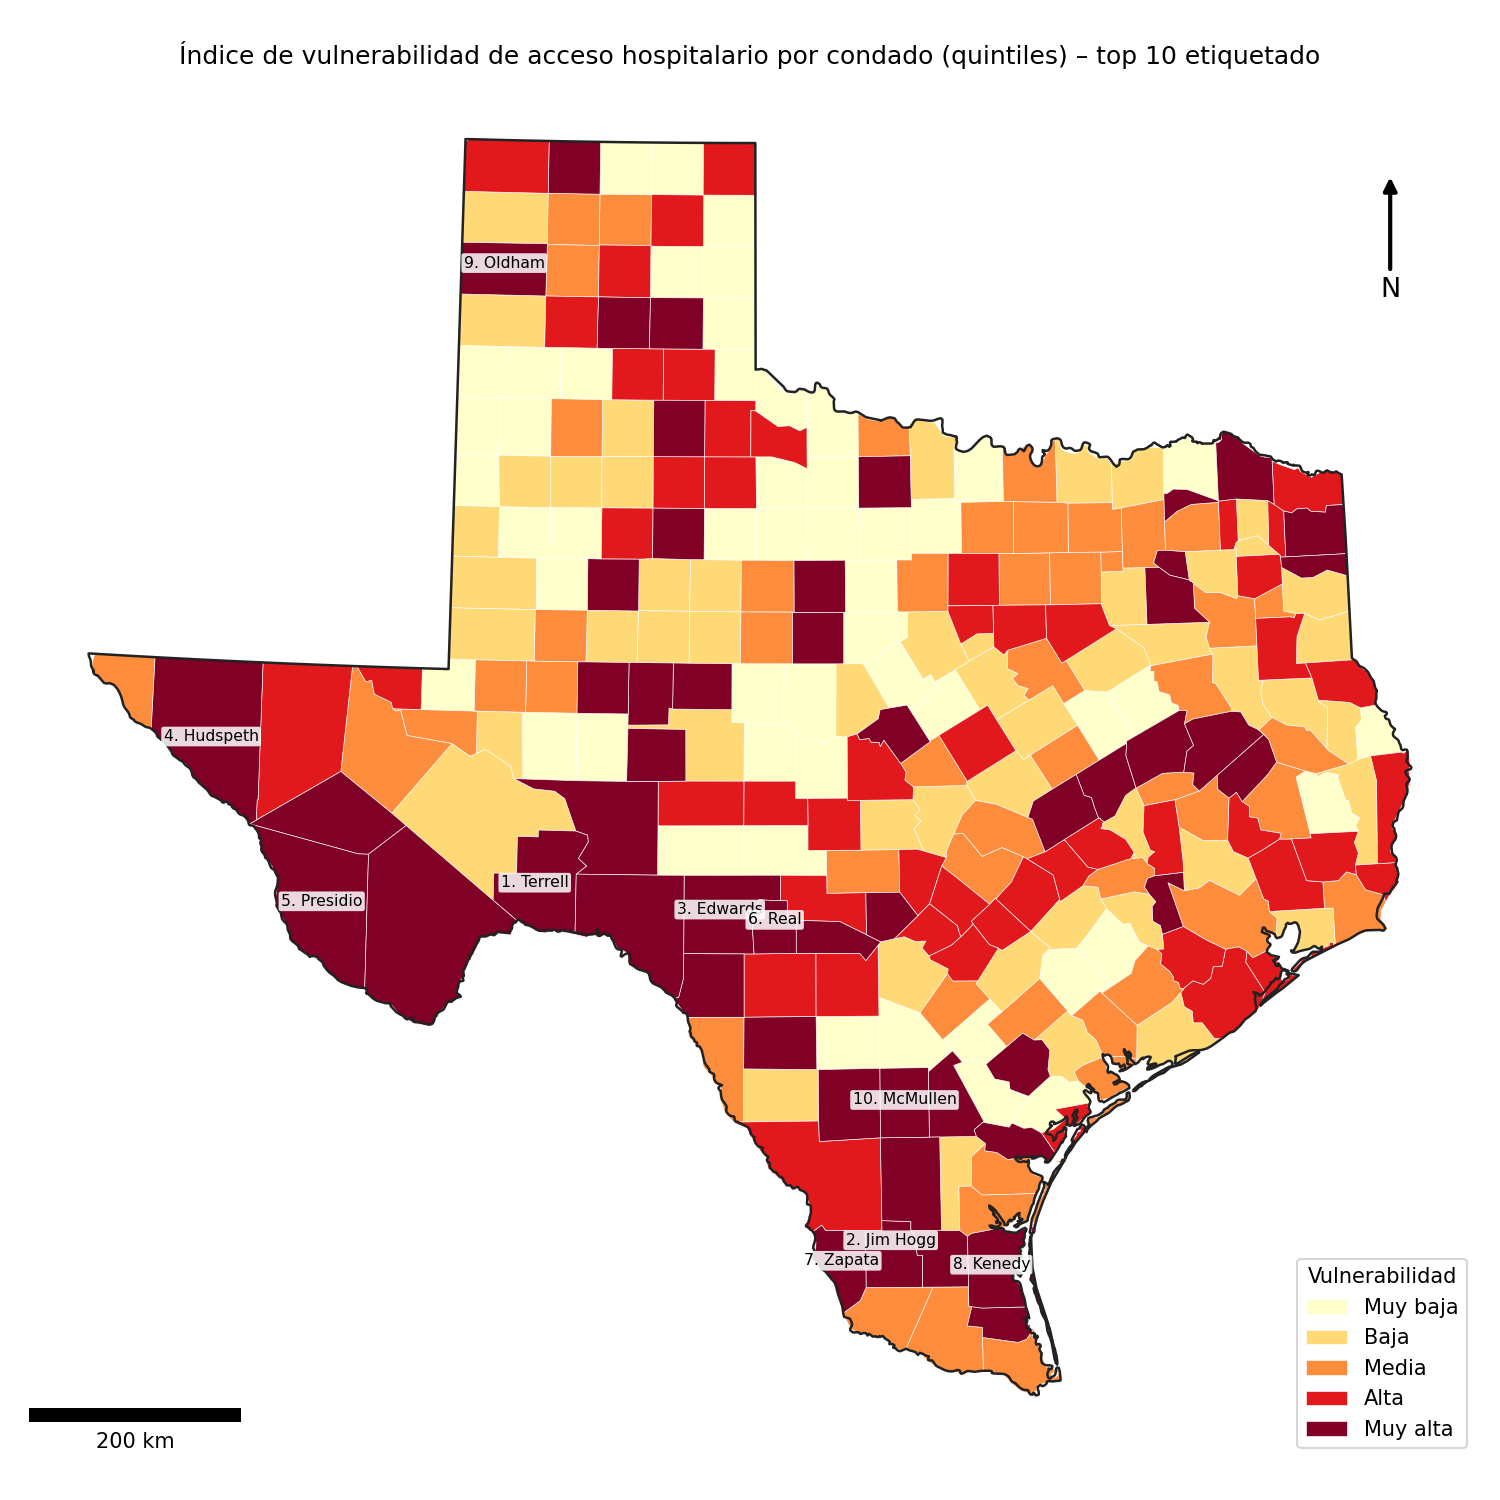
\includegraphics[width=0.9\textwidth]{indice_vulnerabilidad.png}
\caption{Índice de vulnerabilidad por condado (quintiles) con los diez condados más vulnerables etiquetados.}
\end{figure}

Los diez coinciden en nueve de diez con los más alejados del Task 2.1a (Brewster sí tiene un hospital de 25 camas, así que su $C_2$ no es máximo y sale del top 10; entra McMullen). Todos están a más de 64\,km de un hospital, no tienen camas y no tienen ningún hospital con dato de ocupación a 50\,km, por lo que $C_2$ y $C_3$ toman el valor máximo (1.0) en los diez. Consecuencias: dentro de este grupo el orden lo decide solo $C_1$, y el índice \textbf{satura}: distingue entre ``tiene hospital'' y ``no tiene'', pero no entre condados sin hospitales.

%---------------------------------------------------------------------
\subsection{Task 2.3: Optimización de cobertura (MCLP simplificado)}

\paragraph{a) Grilla de candidatos.}
\preg{Genere una grilla regular de candidatos con resolución de 50\,km y elimine los puntos fuera del límite estatal con una intersección espacial.}
\resp{La grilla tiene 650 puntos y \textbf{271 candidatos} quedan dentro de Texas.}
Se generó una grilla regular de 50\,km sobre el rectángulo envolvente del estado: 650 puntos, de los cuales 271 caen dentro del límite estatal (intersección espacial).

\paragraph{b) Población adicional por candidato (radio 25 km).}
\preg{Para cada candidato calcule la población adicional que quedaría cubierta con un radio de 25\,km (población de condados sin cobertura actual que cae dentro del nuevo buffer).}
\resp{Se calculó para los 271 candidatos. La ganancia individual máxima es de 179,382 personas, la mediana es 3,612 y 7 candidatos no aportan nada.}
Para cada candidato se toma la parte de cada condado sin cobertura actual (a 25\,km) y se calcula
\[
\text{Ganancia}(c)=\sum_i \text{Población}_i\times\frac{\text{Área}\big((\text{Condado}_i\setminus C_{25})\cap B(c,25\,\text{km})\big)}{\text{Área}(\text{Condado}_i)}.
\]
La cobertura actual a 25\,km es 87.30\,\%, con 3,683,159 personas sin cobertura. La ganancia individual máxima de un candidato es 179,382 personas (mediana 3,612; 7 candidatos con ganancia 0).

\paragraph{c) Algoritmo voraz (3 hospitales).}
\preg{Implemente un algoritmo voraz que seleccione 3 candidatos que maximicen la cobertura adicional acumulada. Reporte cuánta población adicional cubre cada punto y el porcentaje de cobertura total tras agregar los 3 hospitales. Grafique los 3 puntos sobre el mapa de cobertura final.}
\resp{Los tres sitios elegidos están en los condados de Hidalgo (+179,382 personas), El Paso (+137,429) y Fort Bend (+86,764). En total cubren \textbf{403,575 personas más} y la cobertura a 25\,km pasa de 87.30\,\% a \textbf{88.69\,\%}.}
En cada iteración se elige el candidato con mayor ganancia sobre la población aún sin cobertura, se actualiza el mapa de cobertura y se repite.

\begin{table}[H]
\centering\small
\begin{tabular}{rlrrr}
\toprule
Iteración & Condado del sitio & Población adicional & Adicional acumulada & Cobertura total (\%) \\
\midrule
1 & Hidalgo   & 179,382 & 179,382 & 87.92 \\
2 & El Paso   & 137,429 & 316,811 & 88.39 \\
3 & Fort Bend & 86,764  & 403,575 & 88.69 \\
\bottomrule
\end{tabular}
\end{table}

Tras agregar los 3 hospitales, la cobertura a 25\,km sube de 87.30\,\% a \textbf{88.69\,\%} (403,575 personas más).

\begin{figure}[H]
\centering
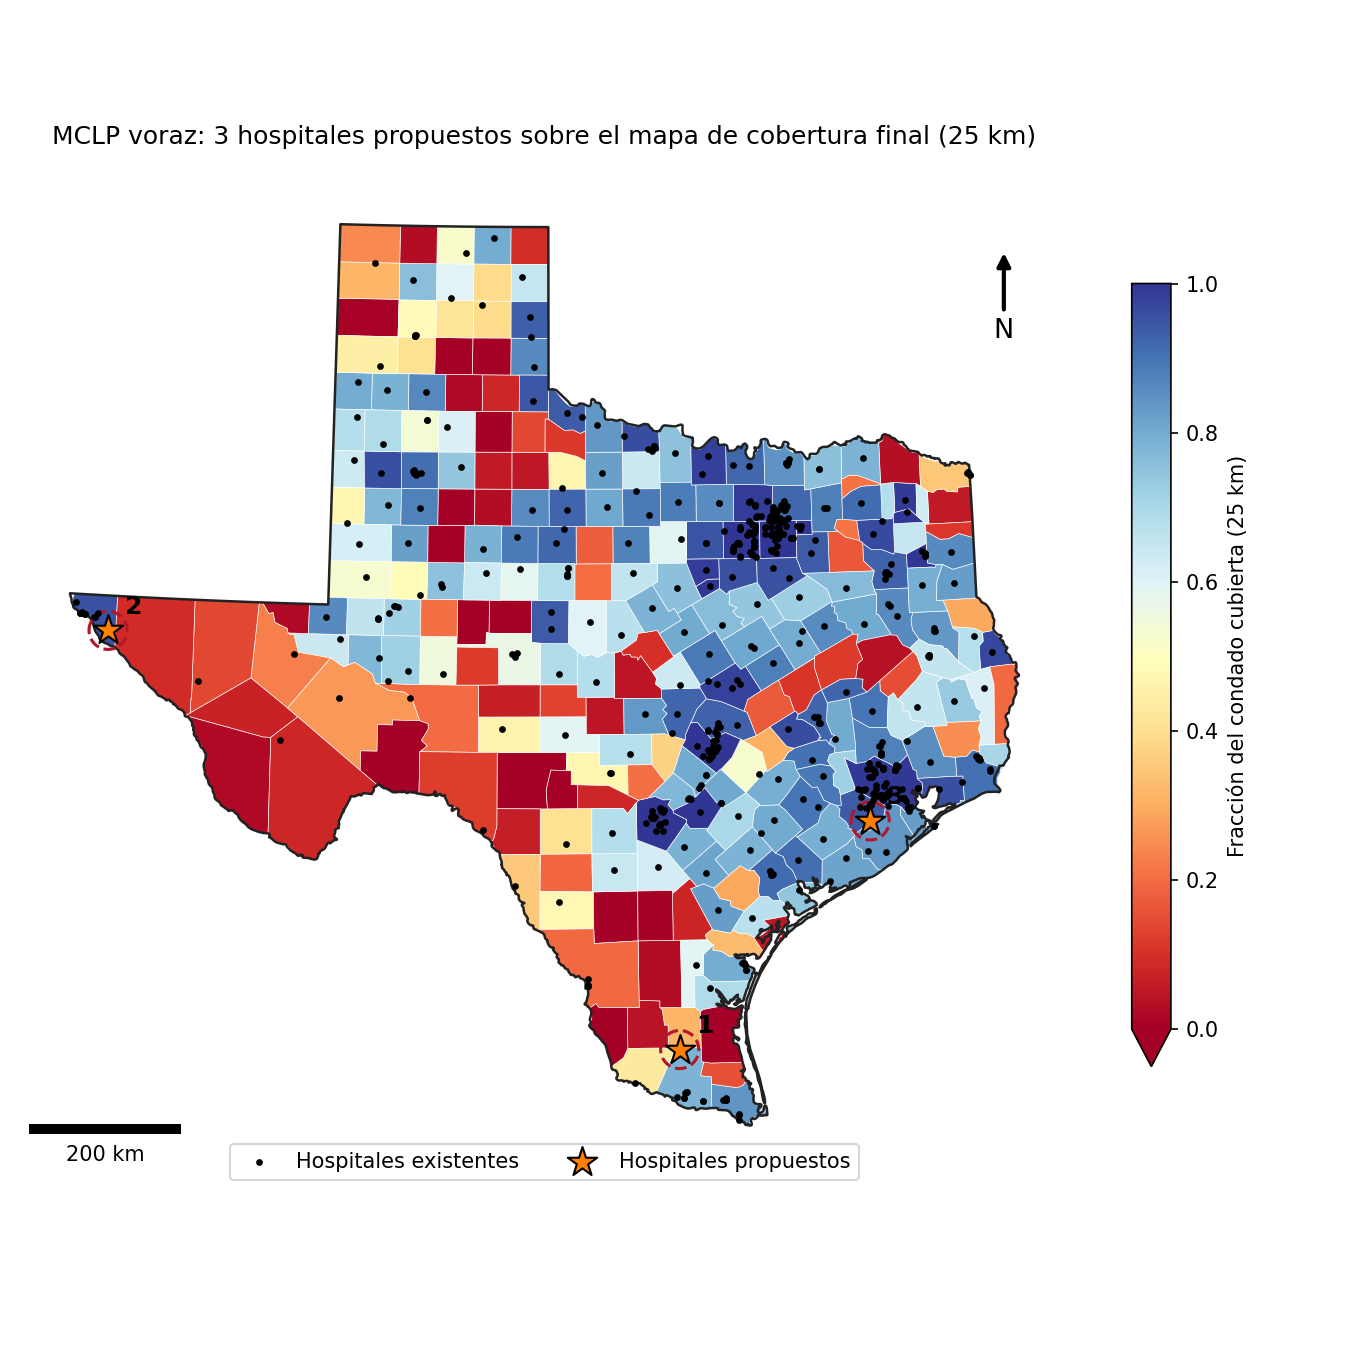
\includegraphics[width=0.85\textwidth]{mclp_voraz.png}
\caption{Los 3 puntos propuestos sobre el mapa de cobertura final a 25\,km.}
\end{figure}

\textbf{Lectura.} Las ganancias decrecen (179 mil, 137 mil, 87 mil), como es de esperar. La mejora es pequeña porque el 87\,\% ya está cubierto y los $\approx3.7$ millones restantes están dispersos en muchos condados parcialmente cubiertos (233 de 254) que tres buffers de 25\,km no alcanzan. Como el modelo asume población uniforme dentro del condado, la parte ``sin cobertura'' de condados grandes y densos (Hidalgo, El Paso, Fort Bend) se supone tan poblada como el resto, aunque en la realidad la gente vive en las ciudades donde ya hay hospitales. Por eso el modelo probablemente \textbf{sobrestima} la población adicional que cubrirían estos sitios y favorece a condados muy poblados frente a zonas rurales remotas. Además, los candidatos están restringidos a una grilla de 50\,km, por lo que los sitios son aproximados.

%=====================================================================
\appendix
\section{Código de carga de los archivos (Task 1.1a)}\label{app:carga}
\begin{verbatim}
import pandas as pd
import geopandas as gpd

hosp_raw = gpd.read_file("hospitales_eeuu.geojson")
cond_raw = gpd.read_file("condados_eeuu.geojson")
est_raw  = gpd.read_file("estados_eeuu.geojson")
pob_raw  = pd.read_csv("poblacion_condados.csv")

archivos = {"hospitales_eeuu.geojson": hosp_raw,
            "condados_eeuu.geojson": cond_raw,
            "estados_eeuu.geojson": est_raw,
            "poblacion_condados.csv": pob_raw}
for nombre, df in archivos.items():
    crs = getattr(df, "crs", None)
    print(nombre, len(df), crs.to_string() if crs else "no aplica")
    print(list(df.columns))
\end{verbatim}

\end{document}
